\documentclass[tikz,border=10pt]{standalone}

\begin{document}
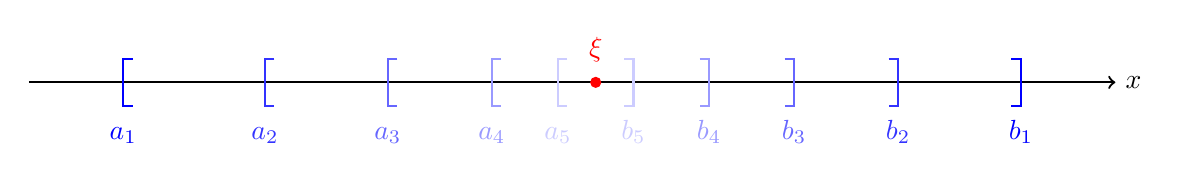
\begin{tikzpicture}[scale=1.2]
    % 绘制数轴
    \draw[->, thick] (-1,0) -- (10.5,0) node[right] {$x$};
    
    % 绘制嵌套区间
    \foreach \a/\b/\c/\n in {
        0.0/9.5/100/1,
        1.5/8.2/80/2,
        2.8/7.1/60/3,
        3.9/6.2/40/4,
        4.6/5.4/20/5%
    } {
        \colorlet{mycolor}{blue!\c}
        
        % 绘制左中括号 "["
        \draw[mycolor, thick] (\a+0.1, 0.25) -- (\a, 0.25) -- (\a, -0.25) -- (\a+0.1, -0.25);
        % 添加了 text height 和 text depth 以统一边界框尺寸
        \node[mycolor, below=2pt, text height=1.5ex, text depth=0.5ex] at (\a, -0.25) {$a_{\n}$};
        
        % 绘制右中括号 "]"
        \draw[mycolor, thick] (\b-0.1, 0.25) -- (\b, 0.25) -- (\b, -0.25) -- (\b-0.1, -0.25);
        \node[mycolor, below=2pt, text height=1.5ex, text depth=0.5ex] at (\b, -0.25) {$b_{\n}$};
    }
    
    % 绘制所有区间的公共极限点 \xi
    \filldraw[red] (5,0) circle (1.5pt) node[above=4pt] {$\xi$};
    
\end{tikzpicture}
\end{document}